\documentclass{ctexart} 

% 封面
\title{简单高效\LaTeX( 吴康隆)学习笔记\thanks{This is a footnote in the title.}}
\author{殷元昊\thanks{This is a footnote in the author.}}
\date{}
            % "\title{title}和"\author{}"是必须定义的,"\date{text}"如果省略,会自动以编译当天的日期为准,如果不想显示日期,可以输入"\date{}"
            % 标题页的脚注用"\thanks{text}"命令完成

% 宏包-----------------------------------------------------------------------------------------------------------------------------------
\usepackage{indentfirst} 
            %* 纯外文环境下,即使使用"\indent"命令,首行也不缩进,可以加载indentfirst宏包解决该问题

% \usepackage{ctex}
            %* 加载ctex宏包也会导致首行缩进

\usepackage[normalem]{ulem}
            % ulem宏包,提供各种下划线和删除线,normalem选项可以防止\emph{}命令的效果变成加下划线

\usepackage{hologo}
            % hologo宏包可以输出许多TeX家族标志


\usepackage{lettrine}
            % 宏包lettrine能够生成首字下沉的效果

% \usepackage{indentfirst}
            %rfr indentfirst宏包强制段首缩进,但是似乎段首一般都会默认缩进。参考这一篇帖子:https://blog.csdn.net/sdu_hao/article/details/103398959,可以发现似乎以前的版本中,LaTeX会默认第一段取消首行缩进,因此这一宏包现在看来已经基本没有存在的必要了

% \usepackage{parskip}
            %rfr 强制所有段首不缩进,参考:https://tex.stackexchange.com/questions/196922/indent-first-paragraph-after-section-and-dont-indent-new-lines

\usepackage{fontspec} 
            % 在XelaTeX编译下,使用fontspec宏包来选择本地安装的字体。注意,该宏包可能会明显增加编译时间

\usepackage[slantfont,boldfont]{xeCJK} 
            % "slantfont"和"bolfont"选项表示允许设置中文的斜体和粗体字形

\setCJKmainfont[boldfont = SimHei]{SimSun} 
            % 设置"SimSun"(宋体)为主要字体,"SimHei"(黑体)为主要字体的粗体字形,即"\textbf{}"或者"{\bfseries}"命令的变换结果。也可以通过slantfont选项来设置主要字体的斜体字行
            %* 各章节的汉字字形也因此发生变化
            %! 注意,"SimSun"和"SimHei"名称中的大小写一定要写对,否则编译会报错

\usepackage{pifont} 
            %* 用于输出图标(symbol fonts)的宏包

\usepackage{xcolor} 
            % 使用xcolor宏包来方便地调用颜色

\usepackage{amsmath} 
            % 宏包amsmath提供了"\eqref"命令,输出默认形式如"(3.1)"所示的数值

% \usepackage{nameref} 
            % nameref宏包不满足于只引用编号,还提供了引用对象的标题内容的功能

\usepackage{lastpage} 
            % lastpage宏包提供的标签"LastPage"可以保证打印出整个文档最后一页的页数

\usepackage[perpage]{footmisc} 
            % footmisc宏包的perpage选项可以让脚注每页重新编号,默认情况下,脚注按章编号

\usepackage{endnotes} 
            % 用于设置尾注的宏包

\usepackage{csquotes} 
            %* 管理在正文中引用文本的宏包

\usepackage[numbers,sort&compress,super,square]{natbib} 
            % 使用natbib宏包可以定制参考文献标号在文中的显示方式
% \usepackage{natbib} 
            %* 只加载natbib宏包,编译会报错
% \usepackage[numbers]{natbib} 
            % 数字编号
            %* 单独设置该选项,编译成功
% \usepackage[sort&compresss]{natbib} 
            % 排序且压缩
            %! 单独设置该选项,编译会报错
% \usepackage[super]{natbib} 
            % 上标
            %* 单独设置该选项,编译成功
% \usepackage[square]{natbib} 
            % 外侧方括号
            %! 单独设置该选项,编译会报错

\usepackage[numbib,numindex]{tocbibind}
            %* "toc"是"table of contents"的缩写  
            %* 使用tocbibind宏包将目录本身、图目录、表目录、索引、参考文献全部编入目录,并且给参考文献章节和索引章节正常编号
            %* 但是并没有专门为图目录和表目录的正常编号设置的可选参数  
% \usepackage[nottoc]{tocbibind} 
            % 目录本身不编入目录
% \usepackage[notlof]{tocbibind} 
            % 图目录不编入目录
% \usepackage[notlot]{tocbibind} 
            % 表目录不编入目录
% \usepackage[notindex]{tocbibind} 
            % 索引不编入目录
% \usepackage[notbib]{tocbibind} 
            % 参考文献不编入目录
% \usepackage[numindex]{tocbibind} 
            % 给索引章节正常编号
% \usepackage[numbib]{tocbibind} 
            % 给参考文献章节正常编号
% \usepackage[none]]{tocbibind} 
            % 禁用所有

\usepackage[section]{placeins}
            % 重新定义了"\section{}"命令,在此之前加上了"\Float-Barrrier"命令,阻止浮动体跨过该位置

\usepackage{graphicx}
            % 使用graphicx宏包和"\includegraphics[options]{name}"命令插入图片

\usepackage{subcaption}
            %* 使用subcaption宏包来创建subfigure环境,在figure环境中嵌套多图
            %! 注意,subcaption宏包和subfig宏包只能加载其中一个,否则编译会报错

% \usepackage{subfig}
            % 使用subfig宏包提供的"\subfloat[sub-caption]{body}"命令,在figure环境中嵌套多图
            %! 注意,subcaption宏包和subfig宏包只能加载其中一个,否则编译会报错 
            
\usepackage{wrapfig}
            % 使用wrapfig宏包进行图文混排

\usepackage{multirow}
            % 使用multirow宏包解决跨行跨列的问题

\usepackage{array} 
            % array宏包提供"m{}"、"b{}"、">{decl}"、"<{decl}"、"!{intercolumn sign}"、"\newcolumntype{name}{definition}"等命令

\usepackage{tabularray} 
            %* tabularray宏包提供使文本靠近表格上端或者下端的命令

\usepackage{makecell} 
            % makecell宏包提供了一种方便在单元格内换行的方式,以及设置水平表线宽度的命令

\usepackage{diagbox} 
            % diagbox宏包提供了分割表头的命令

\usepackage{tabularx} 
            % tabularx宏包的tabularx环境使得表格可以通过在每列上均匀增加列宽的方式设置整表宽度

\usepackage{dcolumn} 
            % dcolumn宏包提供了小数点对齐的对齐方式

\usepackage[twoside]{geometry}
            % 借助geometry宏包进行页面设置
            %* twoside选项会影响到边注命令"\marginpar[left]{right}"中可选参数对应的内容在偶数页上的显示位置,如果不设置twoside选项,则偶数页上的边注都一律显示在右侧,参见"3.5.2 脚注、边注与尾注"一节

\usepackage{fancyhdr}
            % 借助fancyhdr宏包控制页眉和页脚
            %? "hdr"可能是来自"header"的缩写
\pagenumbering{arabic}
            % 设置页码的格式,默认值为arabic,还可以设置为Roman、roman、Alpha、alpha
\pagestyle{fancy}
            % 设置页眉和页脚的格式,还可以设置其他值,包括:empty(无页眉、页脚)、plain(无页眉,页脚只包含一个居中的页码)、headings(无页脚,页眉包含章节编码、章节名称与页码)、myheadings(无页脚,页眉包含页码和用户定义的信息,经检验,默认情况下只包含页眉中的页码)
            %* 在单边模式下,如果不使用"\pagestyle{fancy}"命令,每一页都会显示不带下边线的页眉,不显示页脚,正文部分的第一页和第二页只在页眉的右侧显示页码,从第三页开始,在页眉的左侧显示次节(subsection)编号和次节名称,在页眉的右侧显示页码;如果使用"\pagestyle{fancy}"命令,每一页都会显示包含下边线的页眉以及不带基线的页脚,正文部分的第一页和第二页只在页眉的右侧显示节(section)编号和节名称,在页脚处显示页码,从第三页开始,在页眉的左侧显示次节(subsection)编号和次节名称,在页眉的右侧显示节(section)编号和节名称,在页脚处显示页码
            %* 在双边模式下,如果不使用"\pagestyle{fancy}"命令,奇数页显示不带下边线的页眉,偶数页显示页脚,正文部分的第一页只在页眉的右侧显示页码,正文部分的第二页只在页脚处显示页码,从第三页开始,奇数页在页眉的左侧显示次节(subsection)编号和次节名称,在页眉的右侧显示页码,偶数页在页脚处显示页码;如果使用"\pagestyle{fancy}"命令,每一页都显示带下边线的页眉和不带基线的页脚,正文部分的第一页只在页眉的左侧显示节(section)编号和节名称,在页脚处显示页码,正文部分的第二页只在页眉的右侧显示节(section)编号和节名称,从第三页开始,奇数页在页眉的左侧显示节(section)编号和节名称,在页眉的右侧显示次节(subsection)编号和次节名称,在页脚处显示页码,偶数页在页眉的左侧显示次节(subsection)编号和次节名称,在页眉的右侧显示节(section)编号和节名称,在页脚处显示页码
            %rfr 事实上,上述提到的【节(section)编号和节名称】在页眉和页脚的设置中被属于“较高级别”(higher-level)的信息,【次节(subsection)编号和次节名称】属于“较低级别”(lower-level)的信息,这是在article文档类中的情况,在book文档类中,“较高级别”则是章(chapter),“较低级别”则是节(section),关于页眉和页脚的设置原理的详细介绍,可以参考:https://www.overleaf.com/learn/latex/Articles/How_does_LaTeX_typeset_headers_and_footers%3F#Commands_for_the_output_routine
%* 注意,如果同时设置empty/plain/headings/myheadings参数和以下命令,优先适用前者,以下命令都不会生效,只有将"\pagestyle{}"命令设置为"fancy"参数,以下命令才会生效
% \lhead{} 
%             % 设置页眉左侧的内容,没有内容表示清空默认情况下的内容
% \chead{} 
%             % 设置页眉中间的内容
% \rhead{} 
%             % 设置页眉右侧的内容,没有内容表示清空默认情况下的内容
% \lfoot{} 
%             % 设置页脚左侧的内容
% \cfoot{} 
%             % 设置页脚中间的内容,没有内容表示清空默认情况下的页码
% \rfoot{} 
%             % 设置页脚右侧的内容
\renewcommand{\headrulewidth}{.4pt} 
            % 设置页眉下边线的高度(不是宽度),默认值为0.4pt
\renewcommand{\footrulewidth}{.4pt} 
            % 设置页脚基线的高度(不是宽度),默认值为0pt
% \fancyhf[HOR]{元昊} 
            % 可选参数中可以通过三个字母(大小写均可,前后顺序可以变化)来设置内容位置:H/F代表“页眉/页脚”,E/O代表“偶数页/奇数页”,L/C/R代表“左侧/中间/右侧”
            %* 这一命令相比之前几条设置页眉/页脚的命令,优势在于可以同时设置多个位置的页眉/页脚,并且可以分奇偶页进行设置,也可以单独设置"\fancyhead[places]{header}"或者"\fancyfoot[places]{footer}"
% 也可以通过"\fancypagestyle{style name}{definitions}"命令自定义页眉和页脚格式
% \fancypagestyle{newstyle}{
%     \fancyhf{} % 清空页眉和页脚
%     \fancyhead[c]{\thesection} % 在页眉中间显示节(section)的计数器内容
%     \fancyfoot{\thepage} % 由于没有指定位置,因此在页脚的左中右三个位置处均显示页码
%     }
% \pagestyle{newstyle}

\usepackage{shortvrb}
            % shortvrb宏包支持以一对符号代替"\verb"命令

\usepackage{blindtext}
            %* blindtext宏包提供"\blindtext"命令和"\Blindtext"命令用于生成一段用于测试的文本,提供"\blinddocument"命令和"\Blinddocument"命令用于生成一篇用于测试的带有章节名、列表等内容的文档

% \usepackage{cuted}
            %* cuted宏包提供strip环境,用于解决figure*环境中的图片在双栏模式下无法在首页被插入的问题
            %! 注意,在strip环境中需要使用caption宏包提供的"\captionof{float type}{heading}"命令来设置标题

% \usepackage{dblfloatfix}
            %* dblfloatfix宏包用于解决figure*环境中的图片在双栏模式下无法在底部被插入的问题,但是仍然无法解决图片无法在首页被插入的问题
            %! 注意,dblfloatfix宏包和stfloats宏包不兼容,只能加载其中一个
            %* 但是dblfloatfix宏包可以和nidanfloat宏包兼容

% \usepackage{stfloats} 
            %* stfloats宏包可以同时解决上述两个问题

% \usepackage{nidanfloat} 
            %* nidanfloat宏包也可以同时解决上述两个问题
            %! 注意,加载nidanfloat宏包会导致通过cuted宏包提供的strip环境中的图片消失,但编译不会报错

\usepackage{multicol}
            % multicol宏包提供multicols环境,可以使同一页内分栏与单栏并存,或者分成多栏,但是此时将无法使用不带星号的浮动体和边注
            %! 注意不要将multicols环境和表格中用于合并列的"\multicolumn{n}{cols}{text}"混淆


\usepackage{hyperref}
            % 索引更常用的是hyperref宏包,由于它经常与其他宏包冲突,一般把它放在导言区的最后
            % 加载hyperref宏包后,目录可以实现点击跳转
\hypersetup{colorlinks = true,linkcolor=blue,anchorcolor=blue,citecolor=blue,urlcolor=red}
            % hyperref宏包的选项也可以以"\hypersetup"的形式另起一行书写,colorlinks选项中的默认值是:colorlinks = false,linkcolor = red, anchorcolor = black, citecolor = green, urlcolor = magenta
            %* 如果以上命令作为hyperref宏包的可选参数,应该将其置于必选参数"{hyperref}"的前面,否则设置的可选参数无法生效

% 其他设置------------------------------------------------------------------------------------------------------------------------------------
% 设置大纲深度
% \setcounter{tocdepth}{2}
            %* 大纲在目录中编号到深度2(即"subsection"一级)为止
% \setcounter{secnumdepth}{2}
            %* 大纲在正文中编号到深度2(即"subsection"一级)为止
            %rfr 书中没有说明"tocdepth"和"secnumdepth"的区别,参考:https://texdoc.org/serve/lshort-zh-cn.pdf/0,两者在book/report文档类中的默认值是2(即"subsection"一级),在article文档类中的默认值是3(即"subsubsection"一级)
            %! 注意,如果在正文中使用以上两条命令,尤其对于"tocdepth"来说,要将其放置在"\tableofcontents"命令之前,否则无法对目录产生影响
            %* 还可以发现,计数器名称是不带"\"符号的

% 通过重定义"\the+计数器名称"命令来修改章节编号和表述形式
\renewcommand{\thesection}{第\arabic{section}章}
\renewcommand{\thesubsection}{\arabic{section}.\arabic{subsection}}
\renewcommand{\thesubsubsection}{\arabic{section}.\arabic{subsection}.\arabic{subsubsection}}
            %rfr 重定义计数器的编号和表述形式的命令可以总结成如下结构:\renewcommand{\the+计数器名称}{相关成分+\arabic{计数器名称}+相关成分},关于"\the+<counter-name>"命令和"\arabic{counter-name}"命令这两类命令的不同,可以参见"3.7.1 计数器"一节
            %rfr 重定义"\the+计数器名称"命令不仅可以改变章节编号的数值形式,还可以改变章节名称的表述形式,比如上述命令中将"section"的表述形式从单纯的阿拉伯数字改为了"第+阿拉伯数字+章"的形式,可以参考:https://tex.stackexchange.com/questions/279744/change-the-name-of-sections,但是"subsection"、"subsubsection"也需要进行相应的修改,因为后两者的表述形式中包含了"section"的表述形式(如果还设置了"paragraph"、"subparagraph",则也需要进行相应的修改),可以参见"3.7.1 计数器"一节中关于“调用计数器”部分的介绍
            %* 书中第"3.6.2 大纲与章节"一节中还提到重定义book/report文档类中的"chapter"这一大纲等级的编号和表述形式,但只涉及了"\chaptername"命令,下面简要介绍重定义"chapter"的两个命令:"\chaptername"命令和"\thechapter"命令,使用"\chapter{}"命令,打印出的默认形式是:"Chapter 阿拉伯数字(计数器) + 章名称",其中,"Chapter"是由"\chaptername"控制的,"chapter"以下的"section"、"subsection"等大纲等级不包含这一部分,阿拉伯数字(计数器)是由"\thechapter"命令控制的,可以类比"section"对应的"\thesection"命令等,章名称是由"\chapter{}"命令控制的,因此,重定义"\chaptername"命令改变的是第一部分,重定义"\thechapter"命令改变的是第二部分。"chapter"之上的"part"这一大纲等级的设置也可以参照"chapter"的情况,只不过"\part{}"命令打印出的默认形式是“Part 大写罗马数字(计数器) + 卷名称”

% --------------------------------------------------------------------------------------------------------------------------------------
\begin{document}

% 打印标题
\maketitle

% 通过重定义"\contentsname"命令来修改目录的标题
\renewcommand{\contentsname}{这是目录}
% 目录
\tableofcontents

% 通过重定义"\listfigurename"命令来修改图片目录的标题
\renewcommand{\listfigurename}{这是插图目录}
% 图片目录
\listoffigures

% 通过重定义"\listtablename"命令来修改表格目录的标题
\renewcommand{\listtablename}{这是表格目录}
% 表格目录
\listoftables

\section{写给读者*}
            %? "\section{}"命令中的两个汉字之间的空格在打印时会丢失,暂时不知道什么原因,暂时用"\mbox{}"命令将这两个汉字隔开;后面的“第4章 数学排版”同理;而其他几章“第2章 LaTeX环境配置”、“第3章 LaTeX基础”以及“第5章 LaTeX进阶”中的汉字“章”和英文"LaTeX"之间在打印时存在空格,只不过此处的"LaTeX"是用专用的命令打出的,而经过测试,即使是直接打出来的英文,如果在命令中和其前面的汉字之间存在空格,打印时该空格也会被打印出来。由此看来,这是专属于汉字内部的问题。
            %? 以上问题是在将章名称定为“第一章 写给读者”的情况下产生的
    \subsection{什么是\LaTeX}
    \subsection{\TeX 与\LaTeX 的优缺点}
    \subsection{为什么需要\LaTeX}
    \subsection{MS Word难道不优秀吗}
    \subsection{\LaTeX 生成的文件格式}

\section{\LaTeX 环境配置}
    \subsection{\LaTeX 的使用方法}
        \subsubsection{本地使用:下载\LaTeX 发行版}
        \subsubsection{在线使用:在线\LaTeX 网站}
    \subsection{\TeX Live的安装}
    \subsection{\TeX Live本地宏包的管理*}
    \subsection{\TeX Studio的安装与配置}
    \subsection{\TeX Live的其他使用情况}
        \subsubsection{卸载\TeX Live}
        \subsubsection{更新\TeX Live}
        \subsubsection{更快的\hologo{XeLaTeX} 编译速度*}
    \subsection{编译文档}
	    \subsubsection{尝试第一份文稿}
		    Hello, world ! 

		    你好,世界!

	    \subsubsection{错误的排查}
            Errors(错误):严重的错误

            Warnings(警告):一些不影响生成文档的瑕疵

            Bad Boxes(坏箱):指排版中出现的长度问题。后面的Badness表示错误的严重程度,程度越高数值越大。这类问题需要检查,排除Badness高的选项。坏箱一般不会影响文档的生成,但是文档的排版可能出现问题。

        \subsubsection{\TeX 帮助资源}
        \subsubsection{\TeX 实用工具}

\section{\LaTeX 基础}
    \subsection{认识\LaTeX}
        \subsubsection{命令与环境}
        \subsubsection{保留字符}
            \# 
            \$ 
            \% % 如果在行末添加"%"这个命令,可以防止LaTeX在行末插入一些奇怪的空白符
            \& 
            \_ 
            \{ 
            \} 

        % 以下是输出反斜杠的三种方法
        % 方法一,这一命令两边的数学环境是不可少的,否则会报错        
            $\backslash$

        % 方法二,这一命令不需要数学环境
            \textbackslash

        % 方法三,使用ASCII码进行输出,需要搭配tt字体环境使用,更多符号输出方式可以参考P21
            %* 实际上除了tt字体之外,也可以选择其他字体命令,比如默认的rm字体
            \textrm{\char92}

            {\rmfamily \char92}
            %! 第一种方法、第三种方法输出的反斜杠和第二种方法输出的反斜杠不完全相同:如果将这几种方法输出的反斜杠排列在一行上,会发现第二种方式输出的反斜杠和后面反斜杠符号的间距更小,但是有意思的是,如果将反斜杠后面的符号替换成其他符号,这些反斜杠后的这一间距又会恢复相同,因此在实际情况中,只需要在需要连续使用两个反斜杠符号时,注意选择命令即可,比如,如果要输出"\\"符号,应该选用两个连续的"\textbackslash"命令
            %* 顺便在此可以讨论"\texttt{}"和"{\ttfamily}"这两类不同的命令,这两类命令的大括号的位置和功能是不同的:前一种命令的大括号置于命令之后,是强制性的,用来放置相应的参数,只有大括号内的内容才会受到该命令的影响,其特点有点类似于环境
            %! 如果将这对大括号放置在命令和统辖范围的两边,则该命令只会影响到气候的第一个字符,之后的其它字符则不受影响
            %* 而后一种命令的大括号不是强制性的,如果没有这一对大括号,则该命令之后的所有内容都会受到该命令的影响,如果需要限制该命令影响的范围,则可以在该命令和需要统辖的范围两边加上大括号
            %! 如果只在命令之后的统辖内容的两边加上大括号,则该大括号不会发挥作用,即其后的大括号以外的内容仍然会受到该命令的影响
            %* 下文中会反复出现这两类命令,以下只通过大括号的位置来体现这两类命令的类型,如果没有必要,不再就这一点展开具体讨论

        % 以下是输出类似扬抑符的命令
            \^{} \^a
            %* 该符号如果按照书上所说的命令,单独打印时会报错,需要在后面加上一对大括号,而如果在大括号中填入一个字母(实际可以只填入一个字母而不需要大括号),实际输出的就是一个扬抑符(circumflex)

        % 以下是输出波浪线的几种方法
        % 方法一,这实际是一个数学符号“约等于”(similar)
            $\sim$
            
        % 方法二
            \~{} \~a
            %* 和上文中的^符号一样,该命令如果后面跟上一个字母,实际输出的就是一个波浪号/腭化符(tilde),如果要单独输出这一符号,必须在后面添加一对大括号,在TeXstudio中输出的是一个单独的腭化符,但是在VS Code中输出的就是一个正常的波浪线
            
        % 方法三
            \textasciitilde
            %! 上述命令在不同的编辑器中输出效果不同,在TeXstudio中输出的是一个腭化符,而在VS Code中输出的却是一个正常的波浪线

        \subsubsection{导言区}
            %todo 加表格(\documentclass[options]{style})

        \subsubsection{文件输出}

    \subsection{标点与强调}
        % 大于号和小于号
        %* 以下两种方法输出的都是数学符号中的大于号和小于号
            > < 
            %! TeXstudio中直接输入大于号和小于号不会正确打印相应的符号,但是VS Code中正常,效果等同于两边加上数学环境
            
            $>$ $<$ 
            % 数学符号中的大于号和小于号需要放在数学环境$$中
            
        %* 文本中的大于号和小于号需要使用\textgreater和\textless命令
            \textgreater \textless 
        
            \subsubsection{引号}
            “你好,‘世界’!” 
            % 中文下的单引号和双引号可以用中文输入法直接输入
            
            ``\thinspace`Max' is here.'' 
            % 英文的左单引号是重音符“`”,右单引号是常用的引号符“'”
            %* 英文下的引号嵌套需要借助\thinspace命令分隔
            %* 双引号括起内容中的左单引号和外部左双引号之间的间隔大小:没有任何空格 < 加了\thinspace命令 < 简单的空格
    
        \subsubsection{短横、省略号与破折号}
        % 连字符
            daughter-in-law

        % 数字起止符
            1--2
            
        % 英文破折号
            Listen---I'm serious.
        
        % 中文破折号照常输入即可
            ——
            
        % 中文省略号照常输入即可
            ……
            
        % 英文省略号需要使用\ldots命令
            \ldots
            %* 意即lower dots, v.s. \cdots, 意即center dots
            %? 该命令效果也等同于\dots,但是\ldots在任何模式下都适用,关于dots的相关命令有待探索
            
        % 连打三个句点输出的不是真正的英文省略号
            ...

	    \subsubsection{强调:粗与斜}
            This is the emphasis form of \emph{abc}.
            % 西文的强调命令就是将相应文本转换为斜体,而不是像在中文中将其加粗或者加下划线
    
	    \subsubsection{下划线和删除线}
		% LaTeX原生的加下划线命令
            \underline{abc} 
		
		%以下命令来自ulem宏包,见导言区
            \uline{下划线}\\
            \uuline{双下划线}\\
            \dashuline{虚下划线}\\
            \dotuline{点下划线}\\
            \uwave{波浪线}\\
            \sout{删除线}\\
            %* "sout"来自"strike out"的缩写
            \xout{斜删除线}
            %* "xout"来自"cross out"的缩写
            %rfr 上述每一条命令后面使用了"\\"命令,但是这一条命令的输出效果实际是在同一段之内强制换行,因此在每一条"\\"命令之后的内容都会换行并且顶格打印,而不会空两格,"\newline"命令也具有相同的输出效果。如果需要换行且顶格打印,可以在相应的内容前面使用"\par"命令,或者直接在需要换行处空出一行,参考:https://tex.stackexchange.com/questions/82664/when-to-use-par-and-when-newline-or-blank-lines,书中也在后续的"3.3.1 空格、换行与分段"一节提到了这一问题

        \subsubsection{其他}
    
    \subsection{格式控制}
            \LaTeX 的长度单位:

            \textbf{pt}:point,磅

            \textbf{pc}:pica,1 pc = 12 pt,四号字

            \textbf{in}:inch,英寸,1 in = 72.27 pt

            \textbf{bp}:bigpoint,1 bp = 1/72 in

            \textbf{cm}:centimeter,厘米,1 cm = 1/2.54 in

            \textbf{mm}:millimeter,毫米,1 mm = 1/10 cm

            \textbf{sp}:scaled point,\TeX 的基本长度单位,1 sp = 1/65536 pt

            \textbf{em}:当前字号下,大写字母M的宽度

            \textbf{ex}:当前字号下,小写字母x的高度

            % \textwidth % 页面上文字的总宽度,即页宽减去两侧边距
            % \linewidth % 当前行允许的行宽
            %? 书中没有明确上述两条命令的用法,不过参照下文关于段首缩进长度、段落间距的设置,应该也是和"\setlength{cmd}{length}"命令搭配使用

        \subsubsection{空格、换行与分段}
        % 空格
            Fig.~8
            % "~"命令输出效果等同于一个空格,并且在此空格之后不会换行,这样可以使空格前后内容始终在同一行上

        % 换行和分段
            This is a paragraph (空行). 
            % 之后空一行,空行之后的一行作为新的段落,开头空两格打印
            
            This is another paragraph (\textbackslash par). 
            % 之后不需要空一行,在这一行和下一行之间(通常放在这一行的末尾,或者下一行的开头)的使用"\par"命令,效果等同于空行
            %* 但是即使此处空一行,再在这一行的末尾或者下一行的开头使用"\par"命令,效果也不会有变化
            %rfr 关于空行和"\par"命令在对齐方式和设置行距方面的重要作用,参见"3.3.3 缩进、对齐与行距"一节和"3.4.3 原生字体命令"一节
            \par This is another paragraph. 

            \mbox{}
            % 使用"\mbox{}"命令,并且前一行和后一行都空出,输出效果是打印一个空白段落
            %* "\mbox{}"命令的功能实际上是防止放入其中的词在换行时断开(虽然即使断开也会有连字符连接)
            %* 如果"\mbox{}"命令所在行的前后两行中有一行没有空行,则打印时不会输出空白段落,而是直接开始一个新的段落,即效果等同于空一行
            %? "\mbox{}"中的"m"代表"make",与之相关的另一个命令是"\makebox{}",有待研究

            This is another paragraph (\textbackslash \textbackslash).\\ % 在同一个段落内强制换行,下一行顶格打印
            This is still in the same paragraph (\textbackslash newline).\newline % 效果同上
            This is still in the same paragraph.
            
        % 设置段落间距
            \setlength{\parskip}{0pt plus 1pt} % 默认段落间距
            %rfr 关于默认段落间距,可以参考:https://latexref.xyz/_005cparindent-_0026-_005cparskip.html
            %rfr "0pt plus 1pt"是弹性距离,意即普通情况下是0pt,在有需要的时候可以拉伸到1pt,相应的也可以设置收缩距离(minus),参考:https://github.com/shifujun/UESTCthesis/issues/2
            %* “段落间距”其实就是前一段的最后一行箱子的底部和后一段的第一行箱子之间的顶部之间的距离,关于“箱子”的介绍,可以参见下文关于“基线间距”(行距)的讨论

            set the parskip (default)

            set the parskip (default)

            set the parskip (default)

        % 自定义段落间距
            {\setlength{\parskip}{30pt}
            %* 这一命令如果放到导言区,会导致全文所有的段落间距变为10pt,直到设置新的段落间距为止
            
            set the parskip (30pt)

            set the parskip (30pt)

            set the parskip (30pt)
            }
            %* 该命令的控制对象是统辖范围内的每一段和其前面一段之间的距离(包括统辖范围内的第一段和统辖范围外之前的最后一段之间的距离),因此,不管统辖范围内的最后一段的末尾是否空行或者加上"\par"命令,其和统辖范围外之后的第一段之间的距离都会恢复为原来的长度,因为这个段落间距是由统辖范围外之后的第一段来控制的,下文中行距的设置的也具有类似的特点
            %! "{\setlength{cmd}{length}}"命令作用于统辖范围内的所有段落,不管统辖范围内的最后一段的末尾是否空行或者加上"\par"命令,其和之前一段之间的距离都是该命令设置的长度,即"\setlength{cmd}{length}"命令的效果不依靠每一段最后的空行或者"\par"命令来触发,下文利用该命令来设置段首缩进长度的情况也具有类似的特点

        % 宏包lettrine能够生成首字下沉的效果
            \lettrine{T}{this} is an example. Hope you like this package, and enjoy your \LaTeX\ trip !
            
        \subsubsection{分页}
            \newpage % "\newpage"命令的功能是从当前行开始到当前页的最后不再打印内容,而直接从下一页开始打印后续内容
            \mbox{}
            \newpage
            % 将"\mbox{}"命令和前后两个"\newpage"命令搭配使用,可以达到空出一整页的效果
        
        \subsubsection{缩进、对齐与行距}
        % 设置段首缩进长度
        % 默认段首缩进长度
            set the parindent (default)
        
        % 自定义段首缩进长度
            {\setlength{\parindent}{10em} set the parindent (10em)

            set the parindent (10em)}
            %! 在大括号中的各个段落的段首缩进长度都会受到该命令的影响,并不需要在每个段落的末尾空一行或者加上"\par"命令

        % 强制取消缩进
            \noindent set the parindent (no indent)
            %* 这一命令只会影响到其后的一个段落,而不会导致其后所有的段落都取消缩进,也不需要任何大括号来限制其统辖范围

        %* 段首缩进长度恢复默认值
            set the parindent (default)
            %rfr 关于默认段首缩进长度,可以参考:https://tex.stackexchange.com/questions/247441/what-is-the-width-of-the-standard-paragraph-indent-in-latexs-article-class、https://latexref.xyz/_005cparindent-_0026-_005cparskip.html,其中提到,10pt的article(最常见的LaTeX类型)中默认的段首缩进长度为15pt
            %? 但是经过检验,15pt并不是此处的LaTeX类型(ctexart)的默认段首缩进长度,此处的默认段首缩进长度似乎是2em

        % 设置对齐方式
        % 设置方法一
            \begin{flushleft}
                左对齐

                依然左对齐
            \end{flushleft}
            %* 左对齐的同时也就取消了段首缩进,事实上,右对齐和居中对齐同样也取消了段首缩进,只不过不在页面左侧,看不出来

            \begin{flushright}
                右对齐

                依然右对齐
            \end{flushright}

            \begin{center}
                居中对齐

                依然居中对齐
            \end{center}
            %* 上述三条命令都是以环境形式设立的,因此不会影响到环境以外内容的对齐方式,是推荐的设置方式
        
        % 设置方法二
            {\raggedleft 右对齐
            %* "ragged"在此处是“凹凸不平”的意思,以"raggedleft"为例,其意思是文本的左侧是凹凸不平的,意即“右对齐”
            
            依然右对齐

            }

            {\raggedright 左对齐\par
            依然左对齐\par
            }

            {\centering 居中对齐
            \par 依然居中对齐
            
            }
            %* 以上三条命令会导致其后内容的对齐方式都发生改变,直到设置新的对齐方式或者段首缩进长度,因此不推荐使用,书中也提到,"{\centering}"(包括"{\raggedleft}"、"{\raggedright}")命令常常用在环境内部(或者一对花括号内部)
            %! 和上文中的"{\setlength{cmd}{length}}"命令不同,"{\centering}"、"{\raggedleft}"、"{\raggedright}"命令的效果需要依靠在统辖范围内的每一段的末尾空行或者加上"\par"命令来触发,因此,如果最后一段的末尾没有空行或者加上"\par"命令,为这一段设置的对齐方式将无法生效
            %rfr 参考:https://tex.stackexchange.com/questions/354669/par-before-vs-after,而如果使用方法一,最后一段的末尾不需要空行或者添加"\par"命令

        %* 关于行距的设置,参照"3.4.3 原生字体命令"一节

    \subsection{字体与颜色}
        \subsubsection{字族、字系与字形}
            字体(typeface $\sim$ font)
            \begin{itemize}
                \item 字族:宋体、黑体、楷体 v.s. 罗马体、等宽体
                \item 字系和字形:加粗、加斜
                \item 字号:五号、小四号
            \end{itemize}

        \subsubsection{中西文“斜体”}
        \subsubsection{原生字体命令}
            %* 文本系列的命令和字体系列的命令
            %* 文本系列的命令,以"text-"开头,用于临时改变字体,命令的统辖范围用大括号括起来
            %* 字族/字系/字号系列的命令,以"-family/-series/-shape"结尾,会导致其后的所有内容的字族/字系/字号改变,因此需要在命令和统辖范围的两边加上大括号;另外,这类命令放在导言区虽然不会报错,但是不会影响到正文,只有放在正文中,才会对其后的内容产生影响
            %* 以下均使用文本系列的命令
        
        % 设置字族
            默认字族:\familydefault % "lmr"意即"Latin Modern Roman"
            \begin{itemize}
                \item Roman v.s. \textrm{Roman} % 罗马字族
                %* 默认值
                \item Sans Serif v.s. \textsf{Sans Serif} % 无衬线字族(Sans Serif)
                \item Typewriter v.s. \texttt{Typewriter} % 等宽字族(Typewriter)
            \end{itemize}
        
        % 设置字系
            默认字系:\seriesdefault % "m"应该就是"MiddleSeries"的缩写
            \begin{itemize}
                \item BoldSeries v.s. \textbf{BoldSeries} % 粗体字系(BoldSeries)
                \item MiddleSeries v.s. \textmd{MiddleSeries} % 中粗体字系(MiddleSeries)
                %* 默认值
            \end{itemize}

        % 设置字形
            默认字形:\shapedefault %? 暂时不知道"n"代表什么
            \begin{itemize}
                \item Upright v.s. \textup{Upright} % 竖直字形
                %* 区别不明显
                \item Slant v.s. \textsl{Slant} % 斜体字形
                \item Italic v.s. \textit{Italic} % 强调体字形
                %? 书中在"3.4.2 中西文‘斜体’"一节中提到加斜是指某种字族的Italy字系(根据此处的命令,实际应当是字形),而斜体是指Slant字族,可是根据此处的命令,Slant也被看成是字形的一种。不过不管怎么说,西文中表示强调,都是对字体应用Italic字形。
                \item scap v.s. \textsc{scap} % 小号大写体字形
                %* 适用于小写字母
                %* "sc"来自"small cap(ital)s"
            \end{itemize}

        % 自定义字族/字系/字形命令
            % 以下两条命令是等价的
            % \newcommand*{\newrm}[1]{\textrm{#1}}
            % \newcommand*{\newrm}[1]{{\rmfamily #1}}
            %* 关于这两类命令的区别,参见"3.4.3 原生字体命令"一节
             %rfr 更多关于CJK字体的设置,可以参考:https://blog.csdn.net/xiazdong/article/details/8892070

        % 重定义默认字族
            % \renewcommand*{\familydefault}{\rmdefault} % 默认字族为罗马字族(Roman)
            % \renewcommand*{\familydefault}{\sfdefault} % 默认字族改为无衬线字族(Sans Serif)
            % \renewcommand*{\familydefault}{\ttdefault} % 默认字族改为等宽字族(Typewriter)
            % \renewcommand*{\CJKfamilydefault}{\CJKsfdefault}

        % 重定义某个字族下的默认字体
            % \renewcommand*{\rmdefault}{font-name}
            % \renewcommand*{\sfdefault}{font-name}
            % \renewcommand*{\rmdefault}{ptm}
            %rfr "ptm is the name under which the font family “Times” is installed in your LATEX system",参考:https://www.tug.org/pracjourn/2006-1/schmidt/schmidt.pdf
           
        % 相对字号命令
            % 字号的默认值取决于documentclass,比如article的默认值是10pt
            %* 相对字号命令似乎没有对应的文本系列命令
            相对字号命令
            \begin{itemize}
                \item \tiny tiny 
                %? "tiny"虽然是该组命令中最小的字号,可是其在"itemize"环境中打印出来的前面的点却和"large"一样大,暂时不知道原因是什么
                \item \scriptsize scriptsize
                \item \footnotesize footnotesize
                \item \small small
                \item \normalsize normalsize % 相应的字号默认值
                \item \large large
                \item \LARGE LARGE
                \item \huge huge
                \item \Huge Huge
            \end{itemize}

        % 设置字号和行距
            %rfr "\fontsize{size}{skip}"这一命令要求同时设置字号和行距,如果要单独设置行距,可以使用"\linespread{}"命令,参考:https://tex.stackexchange.com/questions/48741/temporarily-increase-line-spacing/48743#48743、https://mirrors.ibiblio.org/CTAN/macros/latex/required/psnfss/psnfss2e.pdf
            % 字号、行距为默认值
            set the fontsize set the fontsize set the fontsize set the fontsize set the fontsize set the fontsize (default)

            % 字号15pt,行距为默认值(1.2倍文字高)
            {\fontsize{15pt}{\baselineskip}{\selectfont set the fontsize set the fontsize set the fontsize set the fontsize set the fontsize set the fontsize
        
            \selectfont set the fontsize set the fontsize set the fontsize set the fontsize set the fontsize set the fontsize (15pt-baselineskip)
            
            }}
            %* 所谓的“行距”在LaTeX中称为“基线间距”(baselineskip),这一称呼建立在LaTeX的另一个重要概念“箱子”(box)的基础之上,基线位于箱子的内部,箱子顶部到基线的距离称为“高度”(height),箱子底部到基线的距离称为“深度”(depth),“行距”这一称呼容易被误认为是【相邻两行文字之间的空白区域的距离】,但其实仔细思考一下就会发现这种说法站不住脚,因为这个“空白区域”并不是一个矩形区域,而是一个由于上下字符的不同而形成的一个不规则的区域,根本无所谓“距离”的概念:这一区域内的上下两端之间的垂直距离是在不断变化的!因此,即使要称呼“行距”,也要意识到其真正所指是相邻两条基线之间的距离。基线间距的默认值是12倍的文字高度(在article文档类中显示为12pt)。另外,要注意“基线间距”的概念是在同一个段落内进行定义的:一个段落箱子其实就是由一层又一层的行箱子堆叠而成,通过"\baselineskip"命令调整基线间距时,上一行箱子的底部和下一行箱子的顶部之间的距离会随之发生变化,而箱子本身的上下边距则不会变化。还有一个值得思考的地方,那就是前文提到的段落间距的默认值一般情况下是0pt(有1pt的拉伸距离),而唯一可能存在0pt的位置就是上一个段落的最后一行的箱子的底部和下一个段落的第一行箱子的顶部之间的距离,又因为上一个段落的最后一行和下一个段落的第一行之间应该相隔同样的基线间距(暂时缺少官方文献的出处,但这似乎是一个在排版中不言自明的常识),可以推得在同一段落内,上一行的箱子的底部和下一行的箱子的顶部也应该是重合的,在这一推论下,还可以发现,基线间距其实就是上一行箱子的“深度”加上下一行箱子的“高度”,所以,默认情况下的基线间距等于箱子的上下边距,也即箱子的上下边距为12pt
            %rfr 关于"\parskip"和"\baselineskip"命令的测试,可以参考文件"Par_Baseline_skip.tex"
            %! "\selectfont"是"\fontsize{size}{skip}{\selectfont}"命令中预先设定好的一个命令名称,用来引出后面需要修改字号和行距的内容,不要错误地将其理解为需要替换为一个具体的字体名称
            %* 类比前文提到的段落间距的设置,该命令的控制对象是统辖范围内的每一行和其前面一行之间的距离(包括统辖范围内第一行和统辖范围外之前的最后一行之间的距离),因此,不管统辖范围内的最后一行的末尾是否空行或者加上"\par"命令,其和统辖范围外之后的第一行之间的距离都会恢复为原来的长度,因为这个行距是由统辖范围外之后的第一行来控制的
            %! 和上文中的"{\setlength{cmd}{length}}"命令不同,而与上文中的"{\centering}"、"{\raggedleft}"、"{\raggedright}"命令类似,"\fontsize{size}{skip}{\selectfont}"命令的效果需要依靠在统辖范围内的每一段的末尾空行或者加上"\par"命令来触发,因此,如果最后一段的末尾没有空行或者加上"\par"命令,为这一段设置的行距将无法生效,而只有设置的字号生效
            %* 因此可以发现,如果要用这一命令设置行距,统辖范围内的第一行和统辖范围外之前的最后一行可以在同一段落内(通过"\\"命令或者"\newline"命令强制换行),但是统辖范围内的最后一行和统辖范围外之后的第一行一定不在同一段落内,因为统辖范围内的最后一行的末尾必须要空行或者加上"\par"命令,否则这一行和之前一行之间设置的行距将无法生效
            %rfr 参考:https://tex.stackexchange.com/questions/148508/how-does-fontsize-work、https://tex.stackexchange.com/questions/48741/temporarily-increase-line-spacing/48743#48743,从后面这篇帖子还可以发现,即使不需要主动地调整行距,当出现类似的用大括号将命令和统辖范围括起来的情况,最好也在每一段的末尾空行或者加上"\par"命令,否则行距可能会被动地发生变化
            %! 书中给出的命令结构是在"\selectfont"命令"和统辖范围的两边加上大括号,经检验,这对大括号可以省去,但是原文没有提到,还需要在整个"\fontsize{size}{skip}{\selectfont}"命令和统辖范围的两边加上大括号,否则该命令会影响其后所有的内容

            % 字号15pt,行距30pt
            {\fontsize{15}{30}\selectfont set the fontsize set the fontsize set the fontsize set the fontsize set the fontsize set the fontsize (15pt-30pt)\par}
            %* 字号和行距的单位"pt"可以省略

            set the fontsize set the fontsize set the fontsize set the fontsize set the fontsize set the fontsize (default)

             %* 总的来说,如果出现用大括号将命令和统辖范围括起来的情况,在每一段(尤其是最后一行)的末尾空行或者加上"\par"命令是最保险的做法,可以避免很多不必要的问题

        \subsubsection{西文字体}
            %todo 加表格(西文字体)
        % 自定义可调整字族的命令
            \newcommand*{\myfont}[2]{{\fontfamily{#1}\selectfont #2}}
            Let's change font to \myfont{lmss}{Palatino} !
            %rfr 书中输入自定义命令时,字族参数选用的是"ppl"(Palatino),但是系统会警告:"LaTeX Font: Font shape `TU/ppl/m/n' undefined (Font)	 using `TU/lmr/m/n' instead." 意即这一字体搭配不存在,参考:https://tex.stackexchange.com/questions/24628/font-shape-undefined-with-latex-and-isodoc,因此虽然能够打印出结果,但是字体没有发生变化,将字族替换为"lmss"(Latin Modern Roman Serif)之后,警告消失,打印出的字体也发生变化

        % 利用本地安装的字体定义新的字族命令
            %* 书中将以下命令放在了fontspec宏包的部分,但是经检验,即使不加载fontspec,以下命令依然可以生效
            \newfontfamily{\lucida}{Lucida Calligraphy} % 第一个参数定义命令名称,第二个参数输入本地的字体名称
            {\lucida This is Lucida Calligraphy.}
            %! 注意,书中将大括号放在了命令后统辖范围的两边,实际应该放在命令和统辖范围的两边,否则后续内容的西文字体都会变成Lucida Calligraphy

            %rfr 更多关于字体的介绍,可以参考:https://www.tug.org/pracjourn/2006-1/schmidt/schmidt.pdf、https://mirrors.ibiblio.org/CTAN/macros/latex/required/psnfss/psnfss2e.pdf

        \subsubsection{中文支持与CJK字体}
        % ctex宏包支持的字体命令
            {\songti 宋体}

            {\heiti 黑体}

            {\fangsong 仿宋}

            {\kaishu 楷书}

            {\yahei 雅黑}

            {\lishu 隶书}

            {\youyuan 幼圆}
            %* 注意,大括号要放在命令和统辖范围两边
            
        % 使用xeCJK宏包设置CJK主要字体及其粗体
            设置CJK主要字体:宋体

            \textbf{设置CJK主要字体的粗体:黑体}
        
        % 自定义新的CJK字族命令
            %* 可以和上文中定义新的西文字族命令的"\newfontfamily{}{}"比对
            \newCJKfontfamily{\songtii}{SimSun}
            %? 书中给出的定义结构是"\newCJKfontfamily[song]\songti{SimSun}","\songti"两边没有加大括号,编译时会报错,另外,不太明白中括号中的"song"的功能是什么,将其删除,不影响该字族命令的定义

            {\songtii 宋体}

        % 临时设置一种CJK字体
            {\CJKfontspec[fakeslant = 0.2,fakebold = 3]{SimSun} 临时字体}
            %? 暂时还没有弄明白中括号中的选项的功能

        \subsubsection{颜色}\label{subsubsec:3.4.6}
        % 使用xcolor宏包定义颜色
            \definecolor{goldenrod}{RGB}{218,165,32}
            {\color{goldenrod}{秋麒麟色}}

        % xcolor宏包预定义的颜色
            {\color{black}{黑色}}
            
            {\color{darkgray}{深灰色}}

            {\color{lime}{酸橙色}}

            {\color{pink}{粉红色}}

            {\color{violet}{紫罗兰色}}

            {\color{blue}{蓝色}}

            {\color{gray}{灰色}}

            {\color{magenta}{品红色/洋红色}}

            {\color{purple}{紫色}}

            {\color{white}{白色}}

            {\color{brown}{棕色}}

            {\color{green}{绿色}}

            {\color{olive}{橄榄色}}

            {\color{red}{红色}}

            {\color{yellow}{黄色}}

            {\color{cyan}{青色}}

            {\color{lightgray}{浅灰色}}

            {\color{orange}{橙色}}

            {\color{teal}{鸭绿色}}

        % 通过“调色”做出新的效果
            {\textcolor{red!70}{70\%红色}}
            %! 书中在改变颜色的内容两边没有加大括号,会导致编译时只有第一个字符的颜色发生改变

            {\textcolor{blue!50!black!20!white}{50\%蓝色20\%黑色\%30白色}}

            {\textcolor{-yellow}{黄色的互补色}}

    \subsection{引用与注释}
        \subsubsection{标签和引用}
        % LaTeX原生命令提供的索引形式
            这是在\ref{subsubsec:3.4.6} 一节设置的标签,这一节的名称是\nameref{subsubsec:3.4.6},这一标签所在的页码是\pageref{subsubsec:3.4.6}
            %* 注意,如果不使用"\section{title}"命令而使用多一个"*"号的"\section*{title}"命令,则计时器功能将关闭,同时也会影响到"\label{}"命令和"\ref{}"命令,无法索引出相应的大纲编号
            %* 书中提到"\nameref{label}"命令由nameref宏包提供,但是经检验,即使不加载nameref宏包,这一命令依然生效,说明这一命令应该已经被LaTeX吸收,或者也许本来就是LaTeX的原生命令
            %rfr 但是这种索引方式仍然需要依靠在相应位置设置标签来完成,如果想要直接索引出相应章节的名称,可以参考:https://tex.stackexchange.com/questions/75168/get-current-section-name-without-label
            
        % amsmath宏包提供的索引形式
            这是在\eqref{subsubsec:3.4.6}一节设置的标签

        % hyperref宏包提供的索引形式
            这是在\autoref{subsubsec:3.4.6}一节设置的标签,这一节的名称是\hyperref[subsubsec:3.4.6]{颜色}

            这是我的\LaTeX 代码的GitHub仓库的链接:\url{https://github.com/yuanyang11510/Yuanhao_LaTeX}(可点击)|| % 打印出可以点击的链接
            \nolinkurl{https://github.com/yuanyang11510/Yuanhao_LaTeX}(不可点击), % 打印出的颜色为黑色,无法点击的链接 
            它的名称是\href{https://github.com/yuanyang11510/Yuanhao_LaTeX}{Yuanhao\_LaTeX} 

        % 重定义hyperref宏包中"\autoref{label}"的索引形式
            \renewcommand*{\subsubsectionautorefname}{小节标题}
            这是重新定义"\textbackslash autoref\{label\}"索引形式过后的\autoref{subsubsec:3.4.6}一节
        
        % lastpage宏包提供的"LastPage"标签
            第\thepage 页,共\pageref{LastPage}页
            
        \subsubsection{脚注、边注与尾注\protect\footnote{This is a footnote in the subsubsection.}} % 大纲中的脚注需要在"\footnote{}"命令前面再加上"\protect"命令
        % 1. 脚注
        % 正文内的脚注
            正文脚注示例\footnote{This is a footnote.}

        % minipage环境内的脚注
            \begin{minipage}{\linewidth}
                minipage环境脚注示例1\footnote{This is a footnote in the minipage.} %直接在minipage环境内使用"\footnote{}"命令

                minipage环境脚注示例2\footnotemark %在minipage环境内使用"\footnotemark"命令,在minipage环境外使用"\footnotetext{text}"命令
            \end{minipage}
            \footnotetext{This is another footnote in the minipage.}
            %rfr 可以发现,在minipage环境中,两种脚注的设置方式都是有效的,但是两种方式打印出来的脚注的显示位置和标号都不一样,参考:https://tex.stackexchange.com/questions/274/can-i-get-a-normal-footnote-in-a-minipage-environment-in-latex-how

        % 表格环境内的脚注
            \begin{tabular}{l}
                表格环境脚注示例1\footnotemark\\
                表格环境脚注示例2\footnotemark
            \end{tabular}
            \footnotetext{你不需要更多。}
            \footnotetext{你还需要更多。}
            % 表格环境内的脚注可以使用"\footnotemark"命令搭配"\footnotetext{text}"命令的方法设置,但不能直接使用"\footnote{}"命令设置
            %* 如果要在表格环境内使用类似"\footnote{}"的命令设置脚注,可以加载tablefootnote宏包
            
            %* 通过以上两种环境的例子,可以发现,使用"\footnotemark"命令搭配"\footnotetext{text}"命令的方法设置的脚注,会视同正文内设置的脚注,出现在正文的底部,并且参与正文脚注的数字编号;而在minipage环境中直接使用"\footnote{}"命令设置的脚注,则只会出现在minipage的底部,并且采用英文字母编号

        % 在大纲或者"\caption{}"命令中使用脚注,需要加"\protect"
            %* 大纲中的脚注见这一小节标题
            % \caption{Title\protect\footnote{This is a footnote in the caption.}}
            %? 以上这一条命令编译时会报错,应该是因为"\caption{}"命令必须放在浮动体环境中才能够生效,比如table环境或者figure环境,但是经检验,在浮动体环境中,该命令最后编译虽然不会报错,但是无法在底部显示脚注,暂时还不知道原因是什么

        % 脚注之间的距离
            % \footnotesep
            %* 可以搭配"\setlength{cmd}{length}"命令使用
            
        % 重定义每页脚注之上的横线的宽度和高度
            % \renewcommand{\footnoterule}{\rule{0.4\columnwidth}{0.4pt}}
            %rfr "\rule{width}{height}"命令的两个参数分别代表需要设置的宽度和高度,可以参考:https://liam.page/2018/01/11/floats-in-LaTeX-multiple-elements-in-a-single-float/
            
        % 调整脚注到正文的间距
            % \setlength{\skip\footins}{0.5cm}
            %? 暂时不知道"footins"中的"ins"是什么含义

        % 2. 边注
            这一行有边注\marginpar[左侧]{右侧}
            % 默认情况下,边注显示在右侧,边注内容由必选参数控制,如果设置可选参数,则边注在偶数页上会显示在左侧,内容由可选参数控制
            %rfr 但是原文没有指出,这一设置需要文档类型是“双边的”(two-sided)的,book类型默认是双边的,而article和report类型默认是单边的(single-sided),可以在"\documentclass[options]{style}"命令中添加"twoside"选项来使后两类文档变为双边类型,参考:https://blog.csdn.net/xovee/article/details/127625198

        % 改变边注的位置
            {这一行有边注\marginpar[左侧]{右侧}
            \reversemarginpar
            
            这一行有边注\marginpar[左侧]{右侧}
            
            }
             % "\reversemarginpar"命令之后的所有内容的边注的位置会和原本的位置相反
            %? 另外,有意思的一点是,如果该命令之前的内容和该命令之间没有空行(即在同一段落内),该内容也会落入该命令的统辖范围,暂时不知道原因是什么
            %! 如果用大括号将该命令和统辖范围括起来,则每一段的末尾都需要空行或者加上"\par"命令来触发"\reversemarginpar"命令生效

            这一行有边注\marginpar[左侧]{右侧}

        % 有关边注的长度命令
            % \marginparwidth % 控制边注的宽
            % \marginparsep % 控制边注到正文的距离
            % \marginparpush % 控制边注之间的最小距离
            %* 可以搭配"\setlength{cmd}{length}"命令使用
            % 前两者也可以通过geometry宏包来设置

        % 3. 尾注
            % 需要endnotes宏包,书中没有过多介绍
            尾注示例\endnote{This is an endnote.}
            %rfr 需要在正文最后使用"\theendnotes"命令来显示所有尾注,参考:https://tex.stackexchange.com/questions/56145/is-there-a-way-to-move-all-footnotes-to-the-end-of-the-document
            
        \subsubsection{援引环境}
        % quote环境
            鲁智深其师有偈言曰:
            \begin{quote}
                逢夏而擒,遇腊而执。

                听潮而圆,见信而寂。
            \end{quote}
            % 援引内容首行不缩进

        % quotation环境
            圆寂之后,其留颂曰:
            \begin{quotation}
                平生不修善果,只爱杀人放火。
                忽地顿开金绳,这里扯断玉锁。

                咦!钱塘江上潮信来,今日方知我是我。
            \end{quotation}
            % 援引内容首行缩进

        % verse环境
            泰戈尔在他的《园丁集》中写道:
            \begin{verse}
                从你眼里频频掷来的刺激,使我的痛苦永远新鲜。


                悬挂缩进(也称为第二行缩进),通过将段落的第一行置于边距,然后缩进段落的每一行来设置段落的第一行。 选择您要在其中添加悬挂缩进的文本。
            \end{verse}
            % 援引内容悬挂缩进,由于书中举的例子的长度太短,因此此处增加一段较长的文字,以显示悬挂缩进的效果

        \subsubsection{摘要}
            \renewcommand{\abstractname}{这是摘要} % 重定义"\abstractname"命令来修改摘要标题
            \begin{abstract}
                \textbf{article}和\textbf{report}文档类支持摘要。在单栏模式下,摘要相当于一个带标题的quotation环境。双栏模式下,摘要相当于\textbackslash section*命令定义的一节。
            \end{abstract}
        
        \subsubsection{参考文献}
            This is a sample text.\cite{author1.year1,author2.year2}

            This is the text following the reference. 

            % 在正文最后使用"thebibliography"环境来显示所有参考文献

    \subsection{正式排版:封面、大纲与目录}
        \subsubsection{封面}
        \subsubsection{大纲与章节}
        % LaTeX的大纲级别
            \LaTeX 的大纲级别:

            \begin{itemize}
                \item \textbackslash part:部分,这个大纲级别不会打断chapter的编号
                \item \textbackslash chapter:章,\textbf{article}的文档类不包含本大纲级别
                \item \textbackslash section:节
                \item \textbackslash subsection:次节,默认\textbf{report/book}文档类中本级别及以下的大纲级别不进行编号,也不纳入目录
                \item \textbackslash subsubsection:小节,默认\textbf{article}文档类中本级别及以下的大纲级别不进行编号,也不纳入目录
                %! 以上两个大纲级别中作者所谓的“默认”情况,可能是行业中的惯例,并不是命令本身的特点,在"3.5.1 标签和引用"一节已经提到,是否编号和纳入目录,以及在设置标签后是否能索引出大纲编号,是由大纲命令中的"*"号控制的。加上"*"号则不进行编号,也不纳入目录
                \item \textbackslash paragraph:段,极少使用
                \item \textbackslash subparagraph:次段,极少使用
            \end{itemize}

        % LaTeX的大纲深度
            \textbf{book/report}文档类的大纲深度:

            \begin{itemize}
                \item \textbackslash part:-1(与\textbf{article}文档类不同)
                \item \textbackslash chapter:0
                \item \textbackslash section:1(以下与\textbf{article}文档类相同)
                \item \textbackslash subsection:2
                \item \textbackslash subsubsection:3
                \item \textbackslash paragraph:4
                \item \textbackslash subparagraph:5
            \end{itemize}

            \textbf{article}文档类的大纲深度:

            \begin{itemize}
                \item \textbackslash part:0 (与\textbf{book/report}文档类不同)
                \item \textbackslash chapter:\textbf{article}文档类不存在这一大纲级别
                \item \textbackslash section:1(以下与\textbf{book/report}类文档相同)
                \item \textbackslash subsection:2
                \item \textbackslash subsubsection:3
                \item \textbackslash paragraph:4
                \item \textbackslash subparagraph:5
            \end{itemize}

        % book文档类还提供以下命令
            % \frontmatter % 前言,页码为小写罗马字母,其后的章节不编号,但生成页眉、页脚和目录项
            % \mainmatter % 正文,页码为阿拉伯数字,其后的章节编号,页眉、页脚和目录项正常生成
            % \backmatter % 后记,页码格式不变,继续计数,章节不编号,但生成页眉、页脚和目录项

        \subsubsection{目录}

    \subsection{计数器与列表}
        \subsubsection{计数器}
            \LaTeX 中的计数器:
            \begin{itemize}
                \item \textbf{章节}:part、chapter、section、subsection、subsubsection、paragraph与subparagraph
                \item \textbf{编号列表}:enumi、enumii、enumiii与enumiv
                \item \textbf{公式和图表}:equation、figure与table
                \item \textbf{其他}:page、footnote与mpfootnote(mpfootnote用于实现minipage环境的脚注)
                    %rfr 注意,"mpfootnote"应该只是minipage环境中脚注的计数器名称,而不是该环境中设置脚注的命令,minipage中有两种方法设置脚注,其中通过"\footnote{}"命令设置的脚注,计数方法是小写英文字母,对应的计数器应当就是mpfootnote,参见"3.5.2 脚注、边注与尾注"一节
            \end{itemize}

        % 通过"\the+计数器名称"命令来调用计数器
            当前所在章节为\thesection、第\thesubsection 节、第\thesubsubsection 次节
            %rfr "\the+计数器名称"命令默认输出的是计数器数值的阿拉伯数字形式,效果等同于"\arabic{计数器名称}"命令,但是两者的本质是不同的:前者可以通过重定义修改计数器的表述形式,比如将"section"的表述形式由单纯的阿拉伯数字修改为“第+阿拉伯数字+章”的形式,可以参见导言区,而后者输出的永远是一个数值,只不过可以通过更换外部命令来调整该数值的格式,可以参见下文的介绍。在重定义前者时,后者是表述“数值”这一部分必不可少的命令
            %! 如果没有在导言区重定义"section"、"subsection"、"subsubsection"等章节的表述形式,此处关于"\thesection"命令的文本内容本来应该写为“当前所在章节为第\thesection 章”,但是由于"section"的表述形式被重定义为了“第+阿拉伯数字+章”,因此直接写为“当前所在章节为\thesection”即可

        % 指定计数器数值格式
            第\arabic{section}节 % 阿拉伯数字

            第\Alph{section}节 % 大写英文字母

            第\alph{section}节 % 小写英文字母

            第\Roman{section}节 % 大写罗马数字

            第\roman{section}节 % 小写罗马数字

            第\chinese{section}节 % 汉字(ctexart文档类特有)
            %* 可以发现,如果在正文中直接调用计数器的数值,使用"\the+计数器名称"命令,如果要通过以上命令指定计数器数值的格式,则直接在以上命令中使用计数器名称即可,否则如果仍然使用"\the+计数器名称"的结构,编译会报错
        
        % 定义一个新的计数器
            \newcounter{parentcounter} %* 先定义父级计数器,再定义子级计数器,如果顺序颠倒,编译会报错
            \newcounter{soncounter}[parentcounter]
            父级计数器:\arabic{parentcounter} % 默认初始值为0
            子级计数器:\arabic{soncounter} % 默认初始值为0

            \setcounter{soncounter}{1} %* 将子级计数器的初始值手动设置为1
            父级计数器:\arabic{parentcounter} % 父级计数器为0
            子级计数器:\arabic{soncounter} % 子级计数器为1

            \addtocounter{soncounter}{1} %* 为子级计数器手动增加1
            父级计数器:\arabic{parentcounter} % 父级计数器为0
            子级计数器:\arabic{soncounter} % 子级计数器为2


            \addtocounter{parentcounter}{1} %* 为父级计数器手动增加1,自己计数器不归零
            父级计数器:\arabic{parentcounter} % 父级计数器为1
            子级计数器:\arabic{soncounter} % 子级计数器为2
            
            \stepcounter{parentcounter} %* 父级计数器步进1,子级计数器归零
            父级计数器:\arabic{parentcounter} % 父级计数器为2
            子级计数器:\arabic{soncounter} % 子级计数器为0
            %* 可以发现,如果没有设置父级计数器,则"\addtocounter{counter}{1}"命令和"\stepcounter{counter}"命令的效果是一样的
            %! 注意,定义的新计数器只能和"\arabic{counter}"类命令搭配使用输出数值,不能像"\section{}"类命令一样具有设置章节名称的功能,也不能通过重定义"\the+计数器名称"的方式来设置计数器数值的表述形式

        \subsubsection{列表}
        % 1. itemize环境
            无序列表:
            \begin{itemize}
                \item 第一项 % 项目符号默认值为圆点(\textbullet)
                \item [-] 第二项 % 项目符号通过可选参数控制
            \end{itemize}

        % 2. enumerate环境
            自动编号列表:
            \begin{enumerate}
                \item 第一项
                \item [张三] 第二项 % 方括号的使用会打断编号,之后的编号顺次推移
                \item 第三项
            \end{enumerate}

        % 3. description环境
            描述列表:
            \begin{description}
                \item[LaTeX] 一个排版系统
                \item[.tex] LaTeX文档扩展名  
            \end{description}
            % 方括号中的内容会加粗显示

    \subsection{浮动体与图表}

        \subsubsection{浮动体}
            %rfr 关于浮动体的相关命令,可以参考文件"Picture.tex"

        \subsubsection{图片}
            %rfr 关于图片的相关命令,可以参考文件"Picture.tex"

        \subsubsection{表格}
            %rfr 关于表格的相关命令,可以参考文件"Table.tex"

        \subsubsection{非浮动体图标和并列图表}
            %rfr 关于并列图表的相关命令,可以参考文件"Picture.tex"

    \subsection{页面设置}
        \subsubsection{纸张、方向和边距}
            %rfr 关于geometry宏包的相关命令,可以参考文件"Geometry.tex"

        \subsubsection{页眉和页脚}
            %rfr 参看导言区关于fancyhdr宏包及相关命令的介绍

    \subsection{抄录与代码环境}
        %* 下面先引用``3.1.2 保留字符''一节以及``3.2 标点与强调''一节中提到的\LaTeX 无法直接通过文本输入打印的字符(只引用文本中使用的符号,而不包括数学环境中的符号;汉语、英语、法语中的名称用"/"符号隔开):
            \begin{itemize}
                \item \#(井号/number sign, hash, hashtag, pound sign/croisillon)
                \item \$(美元符号,金钱符号,比索符号/dollar sign, peso sign/symbole dollar)
                \item \%(百分号/percent signr/pour cent, pour(-)cent)
                \item \&(和号/ampersand, and sign/esperluette)
                \item \_(下横线,独立下划线,底线/free(-)standingunderscore, underline, low line, low dash)
                \item \{\}(大括号,花括号/braces, curly brackets/accolades)
                \item \textbackslash \textrm{\char92} {\rmfamily \char92}(反斜杠,反斜线/backslash,reverse slash, hack, whack, slosh, bash, backslant, etc./contre-oblique, barre oblique inversé, backslash, antislash
                \item \^{}(扬抑符/circumflex/accent circonflexe)
                \item \~{} \textasciitilde(波浪号/tilde/tilde)
                \item \textgreater \textless(大于号、小于号)
            \end{itemize}
        
        % 使用"\verb(*)"命令或者verbatim(*)直接输出这些符号,在相应的命令或者环境中,这些符号在原来编程语言中的功能都会失效,打印出的字体默认为tt字族
            % \verb|# $ % & _ { } \ ^ ~ < >|
            %! 书中提到可以用花括号(即大括号)将抄录内容括起来,但是经检验,这样编译会报错,可以用"{}"、"*"符号以外的符号将抄录内括起来,但是最好不要选用这些抄录内容中的符号,否则会导致末尾的符号的字体发生变化,比如此处选用"|"符号将抄录内容括起来
            %* VS Code中使用这一命令时,虽然编译不会报错,但是会被当成错误(error)而划上红线,因此此处将其注释掉

            \begin{verbatim}
                # $ % & _ { } \ ^ ~ < >
            \end{verbatim}
            %? 使用verbatim环境将抄录内容包起来,但是打印的时候抄录内容的前面和下面一行各自会出现一段空格,前面的空格似乎和verbatim环境在页面中的缩进有关系,下面一行上的空格暂时不知道原因是什么
        
        % 带"*"号的"verb*"命令或者verbatim*环境表示将抄录内容中的空格用"\textvisiblespace"命令表示出来(显示为"␣"符号)
            % \verb*|# $ % & _ { } \ ^ ~ < >|

            \begin{verbatim*}
                # $ % & _ { } \ ^ ~ < >
            \end{verbatim*}

        % shortvrb宏包支持以一对符号代替"\verb"命令
            % \MakeShortVerb |
            % |# $ % & _ { } \ ^ ~ < >|
            %! 即使在上述的命令和相关内容两边加上大括号,选取的符号在之后的内容中将无法再被输出,经检验,如果选择"|"符号,则之后编译不会报错,但是不再会打印出"|"符号,如果选择"?"符号,则之后编译会报错

% 分栏开始-----------------------------------------------------------------------------------------------------------------------------------
        \setlength{\columnsep}{30pt}
            % 设置“栏边距”(双栏的左右边线到中间分隔线之间的距离),默认值是10pt
            %! 注意,这一命令只有放置在"\twocolumn[text]"命令之前才能对栏边距产生影响,这和对"\columnseprule"的设置不一样
    \twocolumn[\blindtext]
            % 可以使用"\twocolumn[text]"命令进行临时分栏,分栏的同时会自动在前一行命令的最后加上"\clearpage"命令,因此分栏一定是另起一页进行
            % 可选参数用于输出双栏上方预留出的单栏区域的内容
        \setlength{\columnseprule}{.4pt}
            % 双栏之间的分隔线宽\度默认值为0pt,一般可以设置为0.4pt
            %! 这一命令即使放置在"\twocolumn[text]"命令之后,也可以对分隔线宽度产生影响
    \subsection{分栏}
            %* 可以发现,如果要在双栏模式下设置章节名,相应的命令需要放置在"\twocolumn[text]"命令之后
            \textbf{第一部分:figure环境}

            这是一段测试文字……这是一段测试文字……这是一段测试文字……这是一段测试文字……这是一段测试文字……这是一段测试文字……这是一段测试文字……这是一段测试文字……这是一段测试文字……这是一段测试文字……这是一段测试文字……这是一段测试文字……这是一段测试文字……

            \newpage 
            % 在双栏模式下,"\newpage"命令的效果是换栏,"\clearpage"命令的效果才是换页
            \begin{figure}[htbp]
                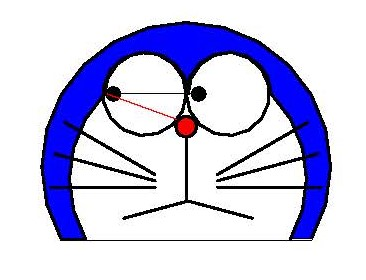
\includegraphics[width = .1\textwidth]{doraemon1.jpg}
                \caption{这是用figure环境在双栏模式下插入的图片(一)}
            \end{figure}
            这是一段测试文字……这是一段测试文字……这是一段测试文字……
            
            \begin{figure}[htbp]
                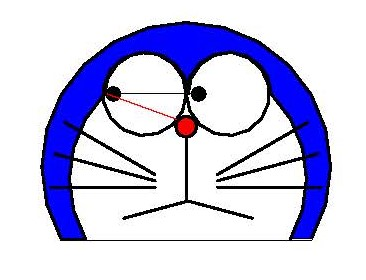
\includegraphics[width = .1\textwidth]{doraemon1.jpg}
                \caption{这是用figure环境在双栏模式下插入的图片(二)}
            \end{figure}
            这是一段测试文字……这是一段测试文字……
            \begin{figure}[htbp]
                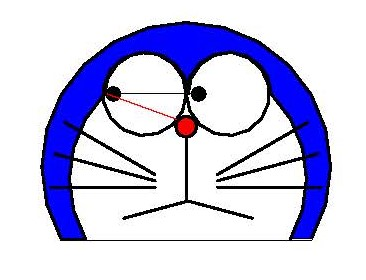
\includegraphics[width = .1\textwidth]{doraemon1.jpg}
                \caption{这是用figure环境在双栏模式下插入的图片(三)}
            \end{figure}
            这是一段测试文字……这是一段测试文字……这是一段测试文字……

            %* 可以发现,在双栏模式下使用figure环境插入图片和在单栏模式下没有什么区别,只不过插入的区域从单栏变成了双栏,插入的图片可以在双栏内部浮动

    \twocolumn
            %* 继续使用一次"\twocolumn[text]"命令,效果是另起一页继续双栏模式
            \textbf{第二部分:figure*环境}

            \begin{figure*}[htbp]
                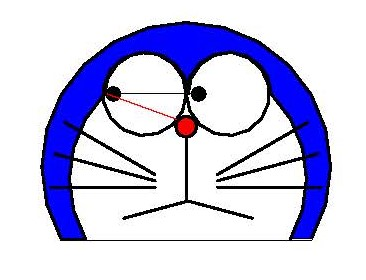
\includegraphics[width = .1\textwidth]{doraemon1.jpg}
                \caption{这是用figure*环境在双栏模式下插入的图片(一)}
            \end{figure*}
            这是一段测试文字……这是一段测试文字……这是一段测试文字……
            
            \begin{figure*}[htbp]
                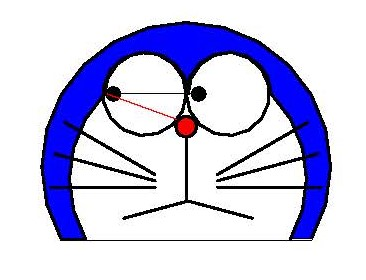
\includegraphics[width = .1\textwidth]{doraemon1.jpg}
                \caption{这是用figure*环境在双栏模式下插入的图片(二)}
            \end{figure*}
            这是一段测试文字……这是一段测试文字……
            \begin{figure*}[htbp]
                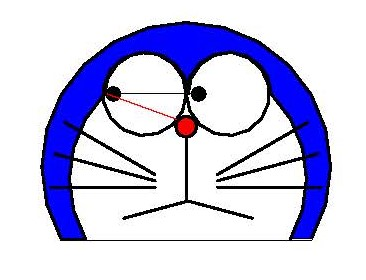
\includegraphics[width = .1\textwidth]{doraemon1.jpg}
                \caption{这是用figure*环境在双栏模式下插入的图片(三)}
            \end{figure*}
            这是一段测试文字……这是一段测试文字……这是一段测试文字……

            \blindtext[7]

            %* 以上做了两步操作:(一)将上一部分的双栏模式中的命令当中的figure环境全部替换为figure*环境,其他命令不变;(二)在原来的命令的末尾加上多行"\blindtext"命令,将双栏中的文本内容填充到三页的篇幅。经过这两步操作后,就会发现很有意思的打印效果:首先,所有的三张图片都被打印到了第二页或者第三页上,尽管这些图片其实很早就被插入进来,尤其是第一张图片,甚至在双栏模式开始之后的第一行就被插入进来,但是其仍然在第二页才被打印出来;其次,这三张图片都被插入进了第二页或者第三页的顶部,因此,可以发现figure*环境在双栏模式下其实并不遵循htbp中的hb规则,而只遵循tp规则(在第一页上似乎只遵循p规则,否则无法解释图片为什么没有被插入第一页的顶部);最后,这些图片被插入的位置并不处于双栏模式下,而是处于单栏模式下,类似于"\twocolumn[text]"命令可选参数的设置效果。结合以上三点,可以发现figure*环境的作用就是在双栏模式下插入【不在双栏内部浮动,而是在每一页的双栏顶部预留出的单栏区域浮动】的图片。这一环境有其存在的合理性:和在双栏模式下的figure环境相比,其可以保证大图在双栏模式下依然拥有足够的插入空间,与双栏模式之外的figure环境相比,其可以保证图片仍然可以插入到双栏文本的内部,而不是只能出现在双栏文本的前面或者后面,table*环境和table环境的区别也可以参照理解。
            %! figure*环境和table*环境中的"*"号和章节命令后面的"*"号代表了完全不同的功能,前者的功能上文已经详述,后者则会导致计数器停止计数,因此,需要意识到,LaTeX中的"*"号并不是一个带有专一功能的记号,而是一个代表在原有命令/环境的基础上改变某些功能的记号
            %rfr 关于上述figure*环境的一些不足之处,多个宏包提出了解决的办法,可以参考文件"Twocolumn.tex"
    \onecolumn
            % 同样可以使用"\onecolumn"命令将双栏模式恢复为单栏模式,与此同时会自动在双栏模式内容的最后加上"\clearpage"命令,因此恢复单栏模式之后的内容会另起一页继续

% 可以使用multicol宏包提供的multicols环境,将页面分成任意多栏
    \begin{multicols}{3}[\centering 这是分成三栏的前言] 
            % 和"\twocolumn[text]"命令的可选参数一样,相应内容会打印在多栏顶部预留出的单栏区域
            \blindtext[2]

            \columnbreak

            \blindtext[2]

            \newpage
            %! 书中提到在该环境下使用"\columnbreak"命令来强制切换到新的一栏,但是经检验,"\newpage"命令依然可以达到相同的效果

            \blindtext[2]
    \end{multicols}

    \blindtext
    \clearpage 
            %* 如果不在multicols环境的后面加上"\clearpage"命令,环境外之后的内容有可能会和多栏处于同一页面上
            %? 这其实会引出一个问题:多栏环境下,系统如何决定多栏的高度?待研究
            %rfr 关于在multicols环境中插入图片,参考文件"Twocolumn.tex"

% 分栏结束------------------------------------------------------------------------------------------------------------------------------------

    \subsection{文档拆分}

    \subsection{西文排版及其他}
        \subsubsection{连写}

        \subsubsection{断词}

        \subsubsection{硬空格与句末标点}

        \subsubsection{特殊符号}

\section{数学排版}

\section{\LaTeX 进阶}

\section[这是目录中显示的标题]{这是正文中显示的标题}
            % 可选参数用于在目录中显示另一个标题,通常是正文中标题的一部分

\section*{不编号的一章}
            %* 该命令设置的章节名称在正文中会打印出来,但是不会编号,在目录中不会打印出来
            \addcontentsline{toc}{section}{不编号的一章}
            %* 该命令设置的章节名称会在目录中打印出来,但是不会编号,在正文中不会打印出来,点击目录中对应的章节名称,索引到该命令在正文中对应的位置,可以发现,该命令类似于一个普通的"\section{}"命令,但是并不会在正文中打印其章节名称
            %! 经检验,上述这一条命令也可以加在除了正文之外的的其他位置,包括导言区,以及"\end{document}"命令之后,编译都不会报错。如果加在导言区,则在目录中会打印在开头,如果加在"\end{document}"之后,则在目录中不会打印出来
            %* 因此,"\section*{title}"命令和"\addcontentsline{file}{secunit}{entry}"命令其实是可以各自独立使用的,但是后者单独使用是没有实际意义的,因为在正文中无法打印出其设置的章节名称。后者实际上只能搭配前者使用,一般将其放置在前者所在的位置之后,这样,在目录中打印出来的章节名称实际上不是前者设置的,而是后者设置的,点击该章节名称实际上也只是索引到后者所在位置,而正文中打印出来的章节名称,则是前者设置的,而不是后者设置的
            %* 结合"\section[short]{title}"命令中可选参数的效果,"\addcontentsline{file}{secunit}{entry}"其实就是将"\section[short]{title}"的可选参数分离出来单独作为一条命令的结果,与之对应的,"\section*{title}"命令就不再含有可选参数,当然,从另一个角度看,"\section*{title}"命令不会在目录中打印章节名,当然没有可选参数存在的必要



    
        % 通过重定义"\refname"命令来修改参考文献的标题
            \renewcommand{\tocbibname}{这是参考文献} 
            % 如果是book类文档,把"\refname"改成"\bibname"
            % 如果加载tocbibind宏包,则修改参考文献标题应该重定义"\tocbibname"命令
            %* 在ctexart文档类型下,参考文献标题默认显示“参考文献”,如果加载tocbibind宏包,依然显示“参考文献”,如果加载natbib宏包,则显示“Bibliography”,如果同时加载natbib宏包和tocbibind宏包,依然显示"Bibliography",可见,tocbibind宏包并不改变参考文献的默认标题,而natbib会将参考文献的标题从默认的“参考文献”修改为"Bibliography",但是只要加载了tocbibind宏包,修改参考文献的标题就要通过重定义"\tocbibname"来完成

        % 显示所有参考文献
            \begin{thebibliography}{99} % “99”表示以最多两位数来编号参考文献,用于对齐
                \addtolength{\itemsep}{-2ex} %? 用于更改行距,"-2ex"代表什么,待研究
                \bibitem{author1.year1}{Au1. ArtName1[J]. JN1. Y:1--2} % 书中在参考文献的形式两边没有加大括号,加与不加,编译的结果相同
                \bibitem{author2.year2}Au2. ArtName2[J]. JN2. Y:1--2
            \end{thebibliography}
            %* 以上都是\LaTeX的原生命令,即使不加载natbib宏包也能编译成功,natbib宏包仅仅是修改了索引的上标形式

        % 显示所有尾注
            \theendnotes

\end{document}

